\chapter{Subcellular Localisation of IFIT1, IFIT3, and IFIT5 in the Context of RSV Inclusion Bodies} \label{ch:Subcellular Localisation of IFIT1, IFIT3, and IFIT5 in the Context of RSV Inclusion Bodies}

\section{Introduction and Aims} \label{sec:Introduction and Aims-Chapter4}
Add intro about what we think it’s happening with IBs and pIBs \newline
Using pIBs as simpler model (only N+P+ cellular components) -> h/bRSV infections -> overexpression during infection


cite qupath for image analysis!!!!!!!!!!!!!


\section{Results} \label{sec:Results-Chapter4}
\subsection{IFIT Subcellular Localisation During Interferon Induction and RSV Infection} \label{subsec:IFIT Subcellular Localisation During Interferon INduction and RSV Infection}
put antibody validation wbs

compare and contrast to the info in databases and papers

% introduction to ib stuff from my study
write about ib size statistics from my analysis


\begin{figure}
    \centering
    \includegraphics[width=1\linewidth]{09. Chapter 4/Figs/01. Localisation introduction/01. IB-zooms.pdf}
    \caption[Representative Infection Zoom.]{\textbf{Representative Infection Zoom.} asdf asdf asdf asdf asdf asdf sdfgsdfg}
    \label{fig:Representative Infection Zoom}
\end{figure}


\begin{figure}
    \begin{subfigure}{0.5\textwidth}
        \includegraphics[width=\textwidth]{09. Chapter 4/Figs/01. Localisation introduction/02. heatmap_all.pdf} 
        \caption[]{Size vs Diameter all}
    \end{subfigure}
    \hfill
    \begin{subfigure}{0.5\textwidth}
        \includegraphics[width=\textwidth]{09. Chapter 4/Figs/01. Localisation introduction/03. heatmap_a549.pdf}
        \caption[]{Size vs Diameter a549}
    \end{subfigure}

    \medskip
    \begin{subfigure}{0.5\textwidth}
        \includegraphics[width=\textwidth]{09. Chapter 4/Figs/01. Localisation introduction/04. heatmap_beas2b.pdf} 
        \caption[]{Size vs Diameter beas2b}
    \end{subfigure}
    \hfill
    \begin{subfigure}{0.5\textwidth}
        \includegraphics[width=\textwidth]{09. Chapter 4/Figs/01. Localisation introduction/05. heatmap_mdbk.pdf} 
        \caption[]{Size vs Diameter mdbk}
    \end{subfigure}
    
    \caption[size vs diameter of ib all and per cell line]{size vs diameter of ib all and per cell line}
    \label{fig:size vs diameter of ib all and per cell line}
    
\end{figure}


% human stuff
Asdfasfsdfasdf \newline
IF Mock | INF | Infection \newline
A549 BEAS2B

Merge pictures of clusters of cells looking at changes between subcellular localisation and a clear increase in mean intensity. Graphs show mean intensity changes from all cells imaged.

\begin{figure}
    \centering
    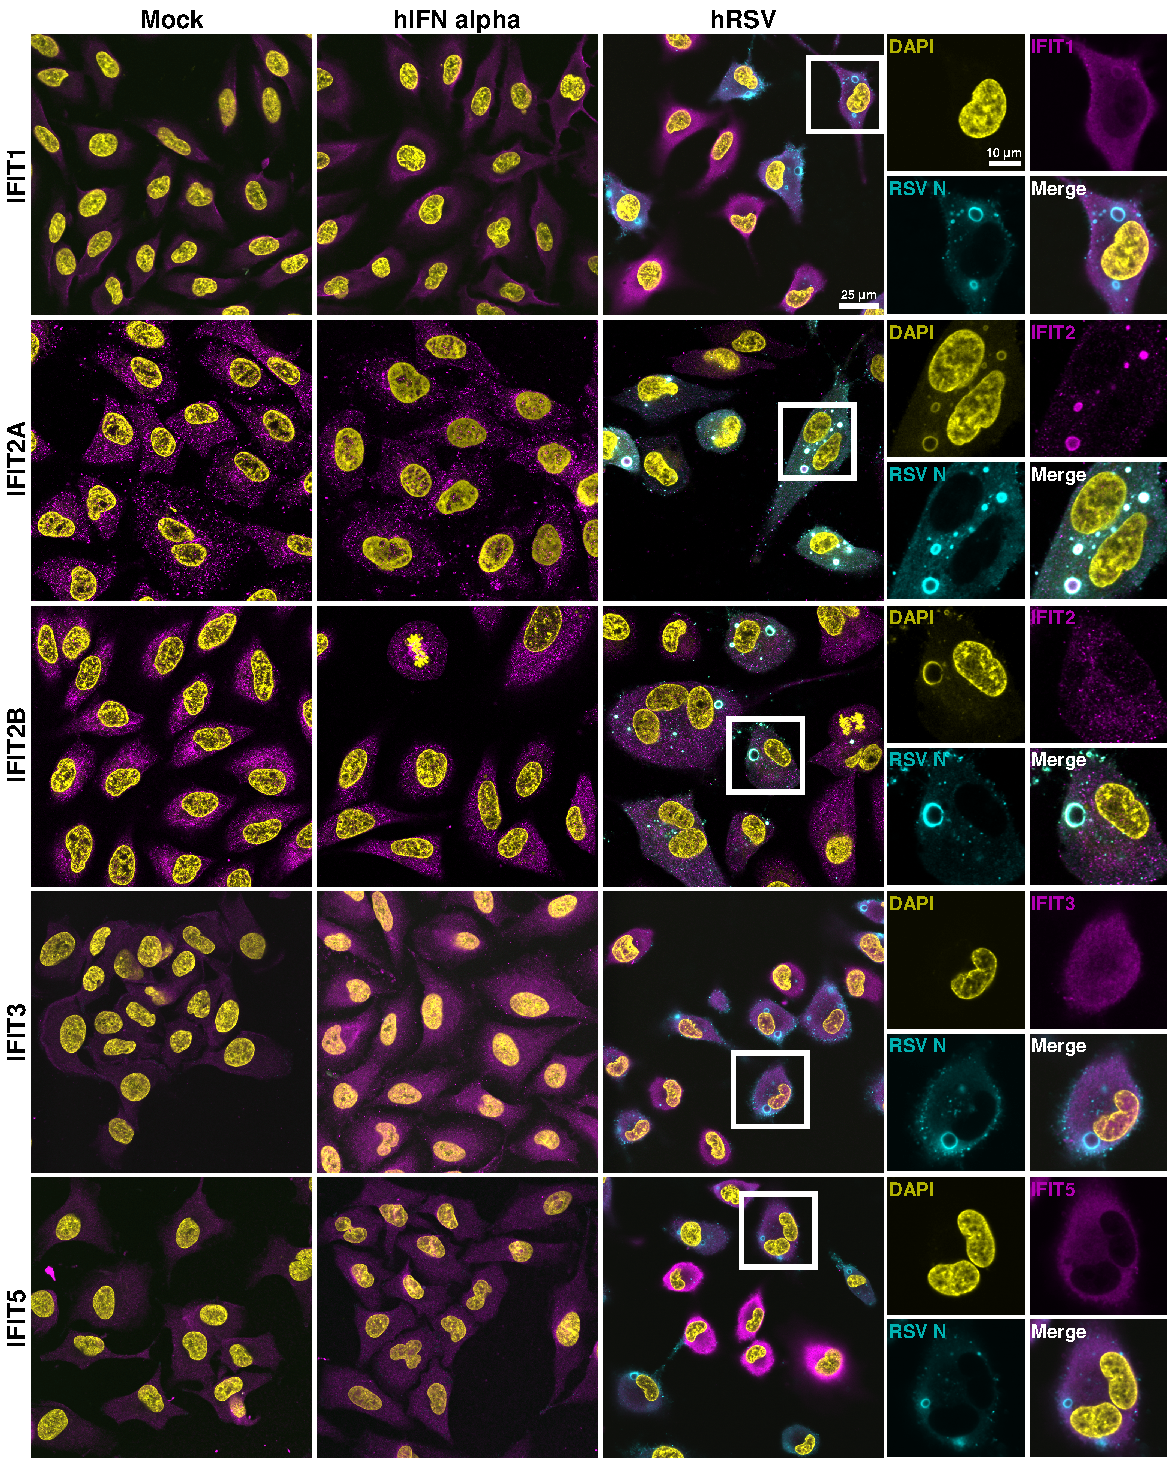
\includegraphics[width=1\linewidth]{09. Chapter 4/Figs/01. Localisation introduction/06. a549 merges.pdf}
    \caption[A549 localisation mergers.]{A549 localisation mergers.}
    \label{fig:A549 localisation mergers.}
\end{figure}


\begin{figure}
    \centering
    \includegraphics[width=1\linewidth]{09. Chapter 4/Figs/01. Localisation introduction/07. a549 plots.png}
    \caption[A549 localisation plots.]{A549 localisation plots.}
    \label{fig:A549 localisation plots.}
\end{figure}


% bovine stuff
Asdfasfsdfasdf \newline
IF Mock | INF | Infection \newline
MDBK BT

Merge pictures of clusters of cells looking at changes between subcellular localisation and a clear increase in mean intensity. Graphs show mean intensity changes from all cells imaged.

\begin{figure}
    \centering
    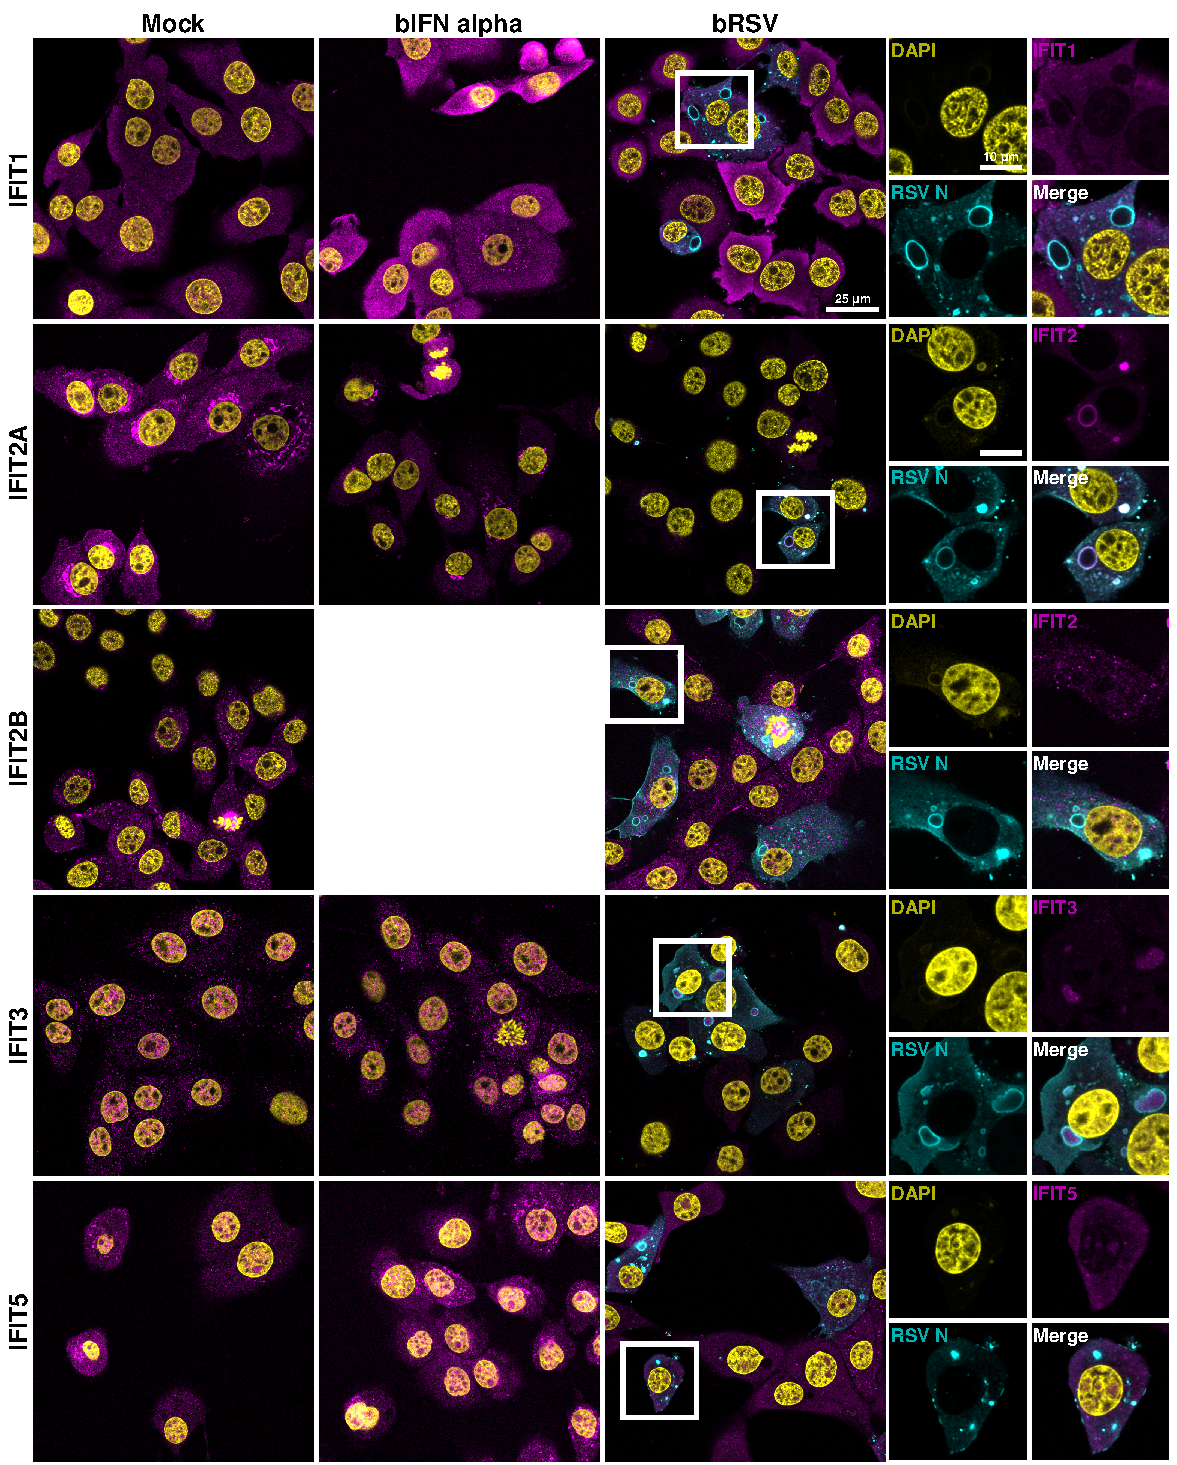
\includegraphics[width=1\linewidth]{09. Chapter 4/Figs/01. Localisation introduction/08. mdbk-merges-test.pdf}
    \caption[MDBK localisation mergers.]{MDBK localisation mergers.}
    \label{fig:MDBK localisation mergers}
\end{figure}


\begin{figure}
    \centering
    \includegraphics[width=1\linewidth]{09. Chapter 4/Figs/01. Localisation introduction/09. mdbk plots.png}
    \caption[MDBK localisation plots.]{MDBK localisation plots.}
    \label{fig:MDBK localisation plots}
\end{figure}

\subsection{Nascent IFIT1, IFIT3, and IFIT5 Localisation During RSV Infection} \label{subsec:Nascent IFIT1, IFIT3, and IFIT5 Localisation During RSV Infection}
\subsubsection{Phenotypic Diversity of Nascent Human and Bovine IFIT1 Interaction with RSV Inclusion Bodies}
Nascent human IFIT1 shows several distinct phenotypes with respect to the hRSV IB interaction. IFIT1 is either concentrated inside the structure (top panel), concentrated on the edge of IB ring (2nd and 3rd panels)  , excluded from the IB structure (4th panel),  or is diffused evenly between the cytoplasm and IB structure (bottom panel).

\begin{figure}
    \begin{subfigure}{0.495\textwidth}
        \caption{}
        \includegraphics[width=1\linewidth]{09. Chapter 4/Figs/02. Infection/01. IFIT1/01. bar_i1_a549.pdf} 
    \end{subfigure}
    \begin{subfigure}{0.495\textwidth}
        \caption{}
        \includegraphics[width=1\linewidth]{09. Chapter 4/Figs/02. Infection/01. IFIT1/02. box_i1_a549.pdf}
    \end{subfigure}
    \caption[Phenotypic Diversity of hIFIT1 Interactions with hRSV Inclusion Bodies in A549 Cell Line.]{\textbf{Phenotypic Diversity of hIFIT1 Interactions with hRSV Inclusion Bodies in A549 Cell Line.} A549 cells were infected with human RSV at MOI 1 and fixed 24 HPI. Cells were double-labeled with with anti-RSV N and anti-IFIT1 antibodies and imaged on confocal microscope. Panel (a) shows percentual proportions of observed phenotypes between hRSV inclusion bodies and hIFIT1 (281 observations), with the red dotted line denoting the 5\% threshold, marking phenotypes considered relevant above this limit. Panel (b) shows the IB area in (\(\mu m^2\)) per observed relevant phenotype.}
    \label{fig:Phenotypic Diversity of hIFIT1 Interactions with hRSV Inclusion Bodies in A549 Cell Line}
\end{figure}

\begin{figure}
    \centering
    \includegraphics[width=1\linewidth]{09. Chapter 4/Figs/02. Infection/01. IFIT1/03. a549 i1.pdf}
    \caption[Representative Images of Phenotypic Diversity of hIFIT1 Interactions with hRSV Inclusion Bodies in A549 Cell Line.]{\textbf{Representative Images of Phenotypic Diversity of hIFIT1 Interactions with hRSV Inclusion Bodies in A549 Cell Line.} A549 cells were infected with hRSV at MOI 1 and fixed at 24 HPI. Cellular nuclei were stained with DAPI (yellow), and cells were double-labeled with anti-RSV N (cyan) and anti-IFIT1 (magenta) antibodies. This figure showcases representative examples of relevant phenotypes in the interaction between hIFIT1 and hRSV inclusion bodies. These phenotypes are presented in descending order based on their percentage proportions. The scale bar indicates 2 (\(\mu m\)).}
    \label{fig:Representative Images of Phenotypic Diversity of hIFIT1 Interactions with hRSV Inclusion Bodies in A549 Cell Line}
\end{figure}

\begin{figure}
    \begin{subfigure}{0.495\textwidth}
        \caption{}
        \includegraphics[width=1\linewidth]{09. Chapter 4/Figs/02. Infection/01. IFIT1/04. bar_i1_beas2b.pdf} 
    \end{subfigure}
    \begin{subfigure}{0.495\textwidth}
        \caption{}
        \includegraphics[width=1\linewidth]{09. Chapter 4/Figs/02. Infection/01. IFIT1/05. box_i1_beas2b.pdf}
    \end{subfigure}
    \caption[Phenotypic Diversity of hIFIT1 Interactions with hRSV Inclusion Bodies in BEAS2B Cell Line.]{\textbf{Phenotypic Diversity of hIFIT1 Interactions with hRSV Inclusion Bodies in BEAS2B Cell Line.} BEAS2B cells were infected with human RSV at MOI 1 and fixed 24 HPI. Cells were double-labeled with with anti-RSV N and anti-IFIT1 antibodies and imaged on confocal microscope. Panel (a) shows percentual proportions of observed phenotypes between hRSV inclusion bodies and hIFIT1 (281 observations), with the red dotted line denoting the 5\% threshold, marking phenotypes considered relevant above this limit. Panel (b) shows the IB area in (\(\mu m^2\)) per observed relevant phenotype.}
    \label{fig:Phenotypic Diversity of hIFIT1 Interactions with hRSV Inclusion Bodies in BEAS2B Cell Line}
\end{figure}

\begin{figure}
    \centering
    \includegraphics[width=1\linewidth]{09. Chapter 4/Figs/02. Infection/01. IFIT1/06. beas2b i1.pdf}
    \caption[Representative Images of Phenotypic Diversity of hIFIT1 Interactions with hRSV Inclusion Bodies in BEAS2B Cell Line.]{\textbf{Representative Images of Phenotypic Diversity of hIFIT1 Interactions with hRSV Inclusion Bodies in BEAS2B Cell Line.} BEAS2B cells were infected with hRSV at MOI 1 and fixed at 24 HPI. Cellular nuclei were stained with DAPI (yellow), and cells were double-labeled with anti-RSV N (cyan) and anti-IFIT1 (magenta) antibodies. This figure showcases representative examples of relevant phenotypes in the interaction between hIFIT1 and hRSV inclusion bodies. These phenotypes are presented in descending order based on their percentage proportions. The scale bar indicates 2 (\(\mu m\)).}
    \label{fig:Representative Images of Phenotypic Diversity of hIFIT1 Interactions with hRSV Inclusion Bodies in BEAS2B Cell Line}
\end{figure}

Nascent bovine IFIT1 in the context of bRSV infection has been observed to localise with the respect of IB in three distinct spaces. We observed it either concentrated inside the central point of the IB structure, while having reduced signal on the inner IB edge, compared to the cytoplasm (top and bottom panels), being excluded from the IB structure (3rd panel), or colocalising on the inner edge of the IB structure while having reduced signal in the middle of the structure compared to cytoplasm, or the edge staining (2nd panel).

\begin{figure}
    \begin{subfigure}{0.495\textwidth}
        \caption{}
        \includegraphics[width=1\linewidth]{09. Chapter 4/Figs/02. Infection/01. IFIT1/07. bar_i1_mdbk.pdf} 
    \end{subfigure}
    \begin{subfigure}{0.495\textwidth}
        \caption{}
        \includegraphics[width=1\linewidth]{09. Chapter 4/Figs/02. Infection/01. IFIT1/08. box_i1_mdbk.pdf}
    \end{subfigure}
    \caption[Phenotypic Diversity of bIFIT1 Interactions with bRSV Inclusion Bodies in MDBK Cell Line.]{\textbf{Phenotypic Diversity of bIFIT1 Interactions with bRSV Inclusion Bodies in MDBK Cell Line.} MDBK cells were infected with bovine RSV at MOI 1 and fixed 24 HPI. Cells were double-labeled with with anti-RSV N and anti-IFIT1 antibodies and imaged on confocal microscope. Panel (a) shows percentual proportions of observed phenotypes between bRSV inclusion bodies and bIFIT1 (117 observations), with the red dotted line denoting the 5\% threshold, marking phenotypes considered relevant above this limit. Panel (b) shows the IB area in (\(\mu m^2\)) per observed relevant phenotype.}
    \label{fig:Phenotypic Diversity of bIFIT1 Interactions with bRSV Inclusion Bodies in MDBK Cell Line}
\end{figure}

\begin{figure}
    \centering
    \includegraphics[width=1\linewidth]{09. Chapter 4/Figs/02. Infection/01. IFIT1/09. mdbk i1.pdf}
    \caption[Representative Images of Phenotypic Diversity of bIFIT1 Interactions with bRSV Inclusion Bodies in MDBK Cell Line.]{\textbf{Representative Images of Phenotypic Diversity of bIFIT1 Interactions with bRSV Inclusion Bodies in MDBK Cell Line.} MDBK cells were infected with bRSV at MOI 1 and fixed at 24 HPI. Cellular nuclei were stained with DAPI (yellow), and cells were double-labeled with anti-RSV N (cyan) and anti-IFIT1 (magenta) antibodies. This figure showcases representative examples of relevant phenotypes in the interaction between bIFIT1 and bRSV inclusion bodies. These phenotypes are presented in descending order based on their percentage proportions. The scale bar indicates 2 (\(\mu m\)).}
    \label{fig:Representative Images of Phenotypic Diversity of bIFIT1 Interactions with bRSV Inclusion Bodies in MDBK Cell Line}
\end{figure}

\subsubsection{Phenotypic Diversity of Nascent Human and Bovine IFIT3 Interaction with RSV Inclusion Bodies}
Nascent human IFIT3 seems to have mainly diffused phenotype (top and bottom panel) with occasional exclusion without any marked IFIT3 concentration adjacent to the IB structure (middle panel).

\begin{figure}
    \begin{subfigure}{0.495\textwidth}
        \caption{}
        \includegraphics[width=1\linewidth]{09. Chapter 4/Figs/02. Infection/02. IFIT3/01. bar_i3_a549.pdf} 
    \end{subfigure}
    \begin{subfigure}{0.495\textwidth}
        \caption{}
        \includegraphics[width=1\linewidth]{09. Chapter 4/Figs/02. Infection/02. IFIT3/02. box_i3_a549.pdf}
    \end{subfigure}
    \caption[Phenotypic Diversity of hIFIT3 Interactions with hRSV Inclusion Bodies in A549 Cell Line.]{\textbf{Phenotypic Diversity of hIFIT3 Interactions with hRSV Inclusion Bodies in A549 Cell Line.} A549 cells were infected with human RSV at MOI 1 and fixed 24 HPI. Cells were double-labeled with with anti-RSV N and anti-IFIT3 antibodies and imaged on confocal microscope. Panel (a) shows percentual proportions of observed phenotypes between hRSV inclusion bodies and hIFIT3 (80 observations), with the red dotted line denoting the 5\% threshold, marking phenotypes considered relevant above this limit. Panel (b) shows the IB area in (\(\mu m^2\)) per observed relevant phenotype.}
    \label{fig:Phenotypic Diversity of hIFIT3 Interactions with hRSV Inclusion Bodies in A549 Cell Line}
\end{figure}

\begin{figure}
    \centering
    \includegraphics[width=1\linewidth]{09. Chapter 4/Figs/02. Infection/02. IFIT3/03. a549 i3.pdf}
    \caption[Representative Images of Phenotypic Diversity of hIFIT3 Interactions with hRSV Inclusion Bodies in A549 Cell Line.]{\textbf{Representative Images of Phenotypic Diversity of hIFIT3 Interactions with hRSV Inclusion Bodies in A549 Cell Line.} A549 cells were infected with hRSV at MOI 1 and fixed at 24 HPI. Cellular nuclei were stained with DAPI (yellow), and cells were double-labeled with anti-RSV N (cyan) and anti-IFIT3 (magenta) antibodies. This figure showcases representative examples of relevant phenotypes in the interaction between hIFIT3 and hRSV inclusion bodies. These phenotypes are presented in descending order based on their percentage proportions. The scale bar indicates 2 (\(\mu m\)).}
    \label{fig:Representative Images of Phenotypic Diversity of hIFIT3 Interactions with hRSV Inclusion Bodies in A549 Cell Line}
\end{figure}

\begin{figure}
    \begin{subfigure}{0.495\textwidth}
        \caption{}
        \includegraphics[width=1\linewidth]{09. Chapter 4/Figs/02. Infection/02. IFIT3/04. bar_i3_beas2b.pdf} 
    \end{subfigure}
    \begin{subfigure}{0.495\textwidth}
        \caption{}        
        \includegraphics[width=1\linewidth]{09. Chapter 4/Figs/02. Infection/02. IFIT3/05. box_i3_beas2b.pdf}
    \end{subfigure}
    \caption[Phenotypic Diversity of hIFIT3 Interactions with hRSV Inclusion Bodies in BEAS2B Cell Line.]{\textbf{Phenotypic Diversity of hIFIT3 Interactions with hRSV Inclusion Bodies in BEAS2B Cell Line.} BEAS2B cells were infected with human RSV at MOI 1 and fixed 24 HPI. Cells were labeled with anti-RSV N and anti-IFIT3 antibodies and imaged on confocal microscope. Panel (a) shows percentual proportions of observed phenotypes between hRSV inclusion bodies and hIFIT3 (16 observations), with the red dotted line denoting the 5\% threshold, marking phenotypes considered relevant above this limit. Panel (b) shows the IB area in (\(\mu m^2\)) per observed relevant phenotype.}
    \label{fig:Phenotypic Diversity of hIFIT3 Interactions with hRSV Inclusion Bodies in BEAS2B Cell Line}
\end{figure}

\begin{figure}
    \centering
    \includegraphics[width=1\linewidth]{09. Chapter 4/Figs/02. Infection/02. IFIT3/06. beas2b i3.pdf}
    \caption[Representative Images of Phenotypic Diversity of hIFIT3 Interactions with hRSV Inclusion Bodies in BEAS2B Cell Line]{\textbf{Representative Images of Phenotypic Diversity of hIFIT3 Interactions with hRSV Inclusion Bodies in BEAS2B Cell Line.} BEAS2B cells were infected with hRSV at MOI 1 and fixed at 24 HPI. Cellular nuclei were stained with DAPI (yellow), and cells were double-labeled with anti-RSV N (cyan) and anti-IFIT3 (magenta) antibodies. This figure showcases representative examples of relevant phenotypes in the interaction between hIFIT3 and hRSV inclusion bodies. These phenotypes are presented in descending order based on their percentage proportions. The scale bar indicates 2 (\(\mu m\)).}
    \label{fig:Representative Images of Phenotypic Diversity of hIFIT3 Interactions with hRSV Inclusion Bodies in BEAS2B Cell Line}
\end{figure}

In this experiment the nascent bovine IFIT3 was consistently concentrated inside IBs. In some IBs the IFIT3 signal showed signs of sub-concentrations within the inclusions (bottom panel; highlighted with arrows), resembling IBAGs (inclusion body associated granules).

Subsequent experiments did not recapitulate the IFIT3 inclusions. It however shows signal which is almost identical to what is observed with IFIT5 in MDBKs during bRSV infection i.e., decrease, but not complete abolishment of IFIT3 signal inside the IB structure (top panel), and IB boundary exclusion while maintaining similar levels of signal intensity between cytoplasmic and intra IB stain.

\begin{figure}
    \begin{subfigure}{0.495\textwidth}
        \caption{}
        \includegraphics[width=1\linewidth]{09. Chapter 4/Figs/02. Infection/02. IFIT3/07. bar_i3_mdbk.pdf} 
    \end{subfigure}
    \begin{subfigure}{0.495\textwidth}
        \caption{}
        \includegraphics[width=1\linewidth]{09. Chapter 4/Figs/02. Infection/02. IFIT3/08. box_i3_mdbk.pdf}
    \end{subfigure}
    \caption[Phenotypic Diversity of bIFIT3 Interactions with bRSV Inclusion Bodies in MDBK Cell Line.]{\textbf{Phenotypic Diversity of bIFIT3 Interactions with bRSV Inclusion Bodies in MDBK Cell Line.} MDBK cells were infected with bovine RSV at MOI 1 and fixed 24 HPI. Cells were labeled with anti-RSV N and anti-IFIT3 antibodies and imaged on confocal microscope. Panel (a) shows percentual proportions of observed phenotypes between bRSV inclusion bodies and bIFIT3 (214 observations), with the red dotted line denoting the 5\% threshold, marking phenotypes considered relevant above this limit. Panel (b) shows the IB area in (\(\mu m^2\)) per observed relevant phenotype.}
    \label{fig:Phenotypic Diversity of bIFIT3 Interactions with bRSV Inclusion Bodies in MDBK Cell Line}
\end{figure}

\begin{figure}
    \centering
    \includegraphics[width=1\linewidth]{09. Chapter 4/Figs/02. Infection/02. IFIT3/09. mdbk i3.pdf}
    \caption[Representative Images of Phenotypic Diversity of bIFIT3 Interactions with bRSV Inclusion Bodies in MDBK Cell Line.]{\textbf{Representative Images of Phenotypic Diversity of bIFIT3 Interactions with bRSV Inclusion Bodies in MDBK Cell Line.} BEAS2B cells were infected with bRSV at MOI 1 and fixed at 24 HPI. Cellular nuclei were stained with DAPI (yellow), and cells were double-labeled with anti-RSV N (cyan) and anti-IFIT3 (magenta) antibodies. This figure showcases representative examples of relevant phenotypes in the interaction between bIFIT3 and bRSV inclusion bodies. These phenotypes are presented in descending order based on their percentage proportions. The scale bar indicates 2 (\(\mu m\)).}
    \label{fig:Representative Images of Phenotypic Diversity of bIFIT3 Interactions with bRSV Inclusion Bodies in MDBK Cell Line}
\end{figure}

\subsubsection{Phenotypic Diversity of Nascent Human and Bovine IFIT5 Interaction with RSV Inclusion Bodies}
hIFIT5 seems to be excluded from hRSV IBs. There is a hint of accumulation of IFIT5 on the outside of IB (bottom panel; no z stacks to confirm this). 

\begin{figure}
    \begin{subfigure}{0.495\textwidth}
        \caption{}
        \includegraphics[width=1\linewidth]{09. Chapter 4/Figs/02. Infection/03. IFIT5/01. bar_i5_a549.pdf} 
    \end{subfigure}
    \begin{subfigure}{0.495\textwidth}
        \caption{}
        \includegraphics[width=1\linewidth]{09. Chapter 4/Figs/02. Infection/03. IFIT5/02. box_i5_a549.pdf}
    \end{subfigure}
    \caption[Phenotypic Diversity of hIFIT5 Interactions with hRSV Inclusion Bodies in A549 Cell Line.]{\textbf{Phenotypic Diversity of hIFIT5 Interactions with hRSV Inclusion Bodies in A549 Cell Line.} A549 cells were infected with human RSV at MOI 1 and fixed 24 HPI. Cells were labeled with anti-RSV N and anti-IFIT5 antibodies and imaged on confocal microscope. Panel (a) shows percentual proportions of observed phenotypes between hRSV inclusion bodies and hIFIT5 (77 observations), with the red dotted line denoting the 5\% threshold, marking phenotypes considered relevant above this limit. Panel (b) shows the IB area in (\(\mu m^2\)) per observed relevant phenotype.}
    \label{fig:Phenotypic Diversity of hIFIT5 Interactions with hRSV Inclusion Bodies in A549 Cell Line}
\end{figure}

\begin{figure}
    \centering
    \includegraphics[width=1\linewidth]{09. Chapter 4/Figs/02. Infection/03. IFIT5/03. a549 i5.pdf}
    \caption[Representative Images of Phenotypic Diversity of hIFIT5 Interactions with hRSV Inclusion Bodies in A549 Cell Line.]{\textbf{Representative Images of Phenotypic Diversity of hIFIT5 Interactions with hRSV Inclusion Bodies in A549 Cell Line.} A549 cells were infected with hRSV at MOI 1 and fixed at 24 HPI. Cellular nuclei were stained with DAPI (yellow), and cells were double-labeled with anti-RSV N (cyan) and anti-IFIT5 (magenta) antibodies. This figure showcases representative examples of relevant phenotypes in the interaction between hIFIT5 and hRSV inclusion bodies. These phenotypes are presented in descending order based on their percentage proportions. The scale bar indicates 2 (\(\mu m\)).}
    \label{fig:Representative Images of Phenotypic Diversity of hIFIT5 Interactions with hRSV Inclusion Bodies in A549 Cell Line}
\end{figure}

\begin{figure}
    \begin{subfigure}{0.495\textwidth}
        \caption{}
        \includegraphics[width=1\linewidth]{09. Chapter 4/Figs/02. Infection/03. IFIT5/04. bar_i5_beas2b.pdf}
    \end{subfigure}
    \begin{subfigure}{0.495\textwidth}
        \caption{}
        \includegraphics[width=1\linewidth]{09. Chapter 4/Figs/02. Infection/03. IFIT5/05. box_i5_beas2b.pdf}
    \end{subfigure}
    \caption[Phenotypic Diversity of hIFIT5 Interactions with hRSV Inclusion Bodies in BEAS2B Cell Line.]{\textbf{Phenotypic Diversity of hIFIT5 Interactions with hRSV Inclusion Bodies in BEAS2B Cell Line.} BEAS2B cells were infected with human RSV at MOI 1 and fixed 24 HPI. Cells were labeled with anti-RSV N and anti-IFIT5 antibodies and imaged on confocal microscope. Panel (a) shows percentual proportions of observed phenotypes between hRSV inclusion bodies and hIFIT5 (21 observations), with the red dotted line denoting the 5\% threshold, marking phenotypes considered relevant above this limit. Panel (b) shows the IB area in (\(\mu m^2\)) per observed relevant phenotype.}
    \label{fig:Phenotypic Diversity of hIFIT5 Interactions with hRSV Inclusion Bodies in BEAS2B Cell Line}
\end{figure}

\begin{figure}
    \centering
    \includegraphics[width=1\linewidth]{09. Chapter 4/Figs/02. Infection/03. IFIT5/06. beas2b i5.pdf}
    \caption[Representative Images of Phenotypic Diversity of hIFIT5 Interactions with hRSV Inclusion Bodies in BEAS2B Cell Line.]{\textbf{Representative Images of Phenotypic Diversity of hIFIT5 Interactions with hRSV Inclusion Bodies in BEAS2B Cell Line.} BEAS2B cells were infected with hRSV at MOI 1 and fixed at 24 HPI. Cellular nuclei were stained with DAPI (yellow), and cells were double-labeled with anti-RSV N (cyan) and anti-IFIT5 (magenta) antibodies. This figure showcases representative examples of relevant phenotypes in the interaction between hIFIT5 and hRSV inclusion bodies. These phenotypes are presented in descending order based on their percentage proportions. The scale bar indicates 2 (\(\mu m\)).}
    \label{fig:Representative Images of Phenotypic Diversity of hIFIT5 Interactions with hRSV Inclusion Bodies in BEAS2B Cell Line}
\end{figure}

The distribution of bIFIT5 is equal between cytoplasmic stain and inside of the IB (with a hint of concentrations/substructures in top and bottom panel; no z stack data available). All 3 panels show a depression of IFIT5 signal at the side of IB boundary (highlighted by arrows).

\begin{figure}
    \begin{subfigure}{0.495\textwidth}
        \caption{}
        \includegraphics[width=1\linewidth]{09. Chapter 4/Figs/02. Infection/03. IFIT5/07. bar_i5_mdbk.pdf} 
    \end{subfigure}
    \begin{subfigure}{0.495\textwidth}
        \caption{}
        \includegraphics[width=1\linewidth]{09. Chapter 4/Figs/02. Infection/03. IFIT5/08. box_i5_mdbk.pdf}
    \end{subfigure}
    \caption[Phenotypic Diversity of bIFIT5 Interactions with bRSV Inclusion Bodies in MDBK Cell Line.]{\textbf{Phenotypic Diversity of bIFIT5 Interactions with bRSV Inclusion Bodies in MDBK Cell Line.} MDBK cells were infected with bovine RSV at MOI 1 and fixed 24 HPI. Cells were labeled with anti-RSV N and anti-IFIT5 antibodies and imaged on confocal microscope. Panel (a) shows percentual proportions of observed phenotypes between bRSV inclusion bodies and bIFIT5 (61 observations), with the red dotted line denoting the 5\% threshold, marking phenotypes considered relevant above this limit. Panel (b) shows the IB area in (\(\mu m^2\)) per observed relevant phenotype.}
    \label{fig:Phenotypic Diversity of bIFIT5 Interactions with bRSV Inclusion Bodies in MDBK Cell Line}
\end{figure}

\begin{figure}
    \centering
    \includegraphics[width=1\linewidth]{09. Chapter 4/Figs/02. Infection/03. IFIT5/09. mdbk i5.pdf}
    \caption[Representative Images of Phenotypic Diversity of bIFIT5 Interactions with bRSV Inclusion Bodies in MDBK Cell Line.]{\textbf{Representative Images of Phenotypic Diversity of bIFIT5 Interactions with bRSV Inclusion Bodies in MDBK Cell Line.} MDBK cells were infected with bRSV at MOI 1 and fixed at 24 HPI. Cellular nuclei were stained with DAPI (yellow), and cells were double-labeled with anti-RSV N (cyan) and anti-IFIT5 (magenta) antibodies. This figure showcases representative examples of relevant phenotypes in the interaction between bIFIT5 and bRSV inclusion bodies. These phenotypes are presented in descending order based on their percentage proportions. The scale bar indicates 2 (\(\mu m\)).}
    \label{fig:Representative Images of Phenotypic Diversity of bIFIT5 Interactions with bRSV Inclusion Bodies in MDBK Cell Line}
\end{figure}

\subsubsection{Summary} \label{Summary-infection}
In the context of infection, endogenous human IFIT1 concentrates within the human RSV IB structure; colocalises to the edge of the IB; is diffused through the structure and cytoplasm equally; or is excluded from the structure. This suggests that the interaction between human IFIT1 and hRSV IB is dynamic and depends on factors that we do not understand yet. In the case of endogenous bovine IFIT1 in the context of bRSV IBs, IFIT1 is either excluded from the structure; excluded from the IB inner edge but concentrated inside; or excluded from the centre of IB structure but concentrated on the inner edge of the structure. 

Nascent human IFIT3 during hRSV infection is either excluded from IB structure or is diffused through the structure. Occasionally it colocalises to the IB ring. Nascent bIFIT3 during bRSV infection either siphons inside IBs and shows sub-IB granules or is excluded from the IB boundary with slightly decreased signal inside of the IB.

In human cells during hRSV infection IFIT5 is mainly excluded from the IBs but seems to concentrate on their edge. Once we saw colocalization with the IB ring and a concentration of IFIT5 inside it. In bovine cells IFIT5 is always excluded from the IB boundary and the signal inside is either slightly decreased or equal compared to cytoplasmic IFIT5. 

\subsection{Nascent IFIT1, IFIT3, and IFIT5 Localisation in a Simplified System of pseudo-IBs} \label{subsec:Nascent IFIT1, IFIT3, and IFIT5 Localisation in a Simplified System of pseudo-IBs}
\subsubsection{pIB IFIT1}
%293t hnhp

\begin{figure}
    \begin{subfigure}{0.5\textwidth}
        \caption{}
        \includegraphics[width=1\linewidth]{09. Chapter 4/Figs/03. pIB/01. IFIT1/01. bar_i1_293t.pdf} 
    \end{subfigure}
    \begin{subfigure}{0.5\textwidth}
        \caption{}
        \includegraphics[width=1\linewidth]{09. Chapter 4/Figs/03. pIB/01. IFIT1/02. box_i1_293t.pdf}
    \end{subfigure}
    \begin{subfigure}{1\textwidth}
        \centering
        \caption{}
        \includegraphics[width=1\linewidth]{09. Chapter 4/Figs/00. placeholder.png}
    \end{subfigure}
    \caption[i1 293t hnhp]{\textbf{i1 293t hnhp.} Nascent bovine IFIT1 in the context of bRSV infection has been observed to localise with the respect of IB in three distinct spaces. We observed it either concentrated inside the central point of the IB structure, while having reduced signal on the inner IB edge, compared to the cytoplasm (top and bottom panels), being excluded from the IB structure (3rd panel), or colocalising on the inner edge of the IB structure while having reduced signal in the middle of the structure compared to cytoplasm, or the edge staining (2nd panel).}
    \label{fig:i1 293t hnhp}
\end{figure}

Detecting magenta: endogenous human IFIT1 \newline
Detecting cyan: human pIB \newline
Cell Line: 293T \newline
Treatment: hNhP \newline

Nascent human IFIT1 seems to be diffused through the pIB structure i.e., the signal intensity and distribution between cytoplasmic and pIB staining is identical.  

%vero hnhp
Detecting magenta: endogenous monkey IFIT1 \newline
Detecting cyan: human pIB \newline
Cell Line: VERO \newline
Treatment: hNhP \newline

Endogenous monkey IFIT1 displays colocalization with human pIB structures (top panel), or inclusion within the structures (bottom panel). Monkey IFIT1 signal is also excluded from the pIB filamentous network (top panel; shown by arrows). This suggests that the colocalization is not caused by mere interaction with N or P but its dependant on the integrity of pIBs. These data are supported by z stack measurements.  

\begin{figure}
    \begin{subfigure}{0.5\textwidth}
        \caption{}
        \includegraphics[width=1\linewidth]{09. Chapter 4/Figs/03. pIB/01. IFIT1/04. bar_i1_vero_hnhp.pdf} 
    \end{subfigure}
    \begin{subfigure}{0.5\textwidth}
        \caption{}
        \includegraphics[width=1\linewidth]{09. Chapter 4/Figs/03. pIB/01. IFIT1/05. box_i1_vero_hnhp.pdf}
    \end{subfigure}
    \caption[i1 vero hnhp plots]{\textbf{i1 vero hnhp plots.} Nascent bovine IFIT1 in the context of bRSV infection has been observed to localise with the respect of IB in three distinct spaces. We observed it either concentrated inside the central point of the IB structure, while having reduced signal on the inner IB edge, compared to the cytoplasm (top and bottom panels), being excluded from the IB structure (3rd panel), or colocalising on the inner edge of the IB structure while having reduced signal in the middle of the structure compared to cytoplasm, or the edge staining (2nd panel).}
    \label{fig:i1 vero hnhp plots}
\end{figure}

\begin{figure}
    \centering
    \includegraphics[width=1\linewidth]{09. Chapter 4/Figs/00. placeholder.png}
    \caption[i1 vero hnhp]{\textbf{i1 vero hnhp.} Nascent bovine IFIT1 in the context of bRSV infection has been observed to localise with the respect of IB in three distinct spaces. We observed it either concentrated inside the central point of the IB structure, while having reduced signal on the inner IB edge, compared to the cytoplasm (top and bottom panels), being excluded from the IB structure (3rd panel), or colocalising on the inner edge of the IB structure while having reduced signal in the middle of the structure compared to cytoplasm, or the edge staining (2nd panel).}
    \label{fig:i3 a549 hrsv}
\end{figure}

%vero bnbp
Cell Line: VERO \newline
Treatment: bNbP \newline
Detecting magenta: endogenous monkey IFIT1 \newline
Detecting cyan: bovine pIB \newline

In the context of bovine pIB structures, nascent monkey IFIT1 seems to colocalise with the edges of the structures (highlighted by the arrows). Consistent to human pIB data, nascent monkey IFIT1 is excluded from filamentous pIB network.

\begin{figure}
    \begin{subfigure}{0.5\textwidth}
        \caption{}
        \includegraphics[width=1\linewidth]{09. Chapter 4/Figs/03. pIB/01. IFIT1/07. bar_i1_vero_bnbp.pdf} 
    \end{subfigure}
    \begin{subfigure}{0.5\textwidth}
        \caption{}
        \includegraphics[width=1\linewidth]{09. Chapter 4/Figs/03. pIB/01. IFIT1/08. box_i1_vero_bnbp.pdf}
    \end{subfigure}
    \begin{subfigure}{1\textwidth}
        \centering
        \caption{}
        \includegraphics[width=1\linewidth]{09. Chapter 4/Figs/00. placeholder.png}
    \end{subfigure}
    \caption[i1 vero bnbp]{\textbf{i1 vero bnbp.} Nascent bovine IFIT1 in the context of bRSV infection has been observed to localise with the respect of IB in three distinct spaces. We observed it either concentrated inside the central point of the IB structure, while having reduced signal on the inner IB edge, compared to the cytoplasm (top and bottom panels), being excluded from the IB structure (3rd panel), or colocalising on the inner edge of the IB structure while having reduced signal in the middle of the structure compared to cytoplasm, or the edge staining (2nd panel).}
    \label{fig:i1 vero bnbp}
\end{figure}

\subsubsection{pIB IFIT3}
%vero hnhp
Detecting magenta: endogenous monkey IFIT3 \newline
Detecting cyan: human pIB \newline
Cell Line: VERO \newline
Treatment: hNhP \newline

Nascent monkey IFIT3 seems to behave a if he pIB was not here. This means I has diffused phenotype. One exception is the top panel (shown with the arrow) which hints at concentrated IFIT3 at the edge of the pIBs. We do not know the localisation with respect to the pIB filaments as none were found in the slides. This data is as well supported by z stack measurements.

\begin{figure}
    \begin{subfigure}{0.5\textwidth}
        \caption{}
        \includegraphics[width=1\linewidth]{09. Chapter 4/Figs/03. pIB/02. IFIT3/01. bar_i3_vero.pdf} 
    \end{subfigure}
    \begin{subfigure}{0.5\textwidth}
        \caption{}
        \includegraphics[width=1\linewidth]{09. Chapter 4/Figs/03. pIB/02. IFIT3/02. box_i3_vero.pdf}
    \end{subfigure}
    \caption[i3 vero hnhp plots]{\textbf{i3 vero hnhp plots.} Nascent bovine IFIT1 in the context of bRSV infection has been observed to localise with the respect of IB in three distinct spaces. We observed it either concentrated inside the central point of the IB structure, while having reduced signal on the inner IB edge, compared to the cytoplasm (top and bottom panels), being excluded from the IB structure (3rd panel), or colocalising on the inner edge of the IB structure while having reduced signal in the middle of the structure compared to cytoplasm, or the edge staining (2nd panel).}
    \label{fig:i3 vero hnhp plots}
\end{figure}

\begin{figure}
    \centering
    \includegraphics[width=1\linewidth]{09. Chapter 4/Figs/00. placeholder.png}
    \caption[i3 vero hnhp]{\textbf{i3 vero hnhp.} Nascent bovine IFIT1 in the context of bRSV infection has been observed to localise with the respect of IB in three distinct spaces. We observed it either concentrated inside the central point of the IB structure, while having reduced signal on the inner IB edge, compared to the cytoplasm (top and bottom panels), being excluded from the IB structure (3rd panel), or colocalising on the inner edge of the IB structure while having reduced signal in the middle of the structure compared to cytoplasm, or the edge staining (2nd panel).}
    \label{fig:i3 vero hnhp}
\end{figure}

\subsubsection{pIB IFIT5}
%vero hnhp
Detecting magenta: endogenous monkey IFIT5 \newline
Detecting cyan: human pIB \newline
Cell Line: VERO \newline
Treatment: hNhP \newline

Nascent monkey IFIT5 colocalises with hRSV pseudo inclusion bodies (basically resembling the P staining). It also colocalises with pIB filamentous network. This network is only seen in cells that are co-transfected with RSV N and P proteins. We believe that they are an aftermath of a pIB breakdown. This data is as well supported by z stack measurements.

\begin{figure}
    \begin{subfigure}{0.5\textwidth}
        \caption{}
        \includegraphics[width=1\linewidth]{09. Chapter 4/Figs/03. pIB/03. IFIT5/01. bar_i5_vero.pdf} 
    \end{subfigure}
    \begin{subfigure}{0.5\textwidth}
        \caption{}
        \includegraphics[width=1\linewidth]{09. Chapter 4/Figs/03. pIB/03. IFIT5/02. box_i5_vero.pdf}
    \end{subfigure}
    \begin{subfigure}{1\textwidth}
        \centering
        \caption{}
        \includegraphics[width=1\linewidth]{09. Chapter 4/Figs/00. placeholder.png}
    \end{subfigure}
    \caption[i5 vero hnhp]{\textbf{i5 vero hnhp.} Nascent bovine IFIT1 in the context of bRSV infection has been observed to localise with the respect of IB in three distinct spaces. We observed it either concentrated inside the central point of the IB structure, while having reduced signal on the inner IB edge, compared to the cytoplasm (top and bottom panels), being excluded from the IB structure (3rd panel), or colocalising on the inner edge of the IB structure while having reduced signal in the middle of the structure compared to cytoplasm, or the edge staining (2nd panel).}
    \label{fig:i5 vero hnhp}
\end{figure}

\subsubsection{Summary} \label{Summary-pib}
Endogenous human IFIT1 seems to be diffused through the human pIB structure. On the other hand, endogenous monkey IFIT1 forms an inclusion in human pIBs, colocalises with the edge of human and bovine pIBs and is excluded from the filamentous pIB network. This suggests that the colocalization is not caused by mere interaction with N or P but its dependant on the integrity of pIBs.

Endogenous monkey IFIT3 seems to be diffuse through the human pIB structures (with maybe a small hint of colocalization).

Endogenous monkey IFIT5 colocalises with human pIBs and with the NP network (this network is never present in infected cells, so we do not know how are other IFIT5s colocalising with it).
\subsection{Exogenous IFIT1, IFIT3, and IFIT5 Localisation  During RSV Infection} \label{subsec:Exogenous IFIT1, IFIT3, and IFIT5 Localisation  During RSV Infection}
\subsubsection{OE IFIT1}
Overexpressed hIFIT1-FLAG colocalises with both human and bovine RSV IBs. This data is supported by evidence from z stacks.

\begin{figure}
    \begin{subfigure}{0.495\textwidth}
        \caption{}
        \includegraphics[width=1\linewidth]{09. Chapter 4/Figs/04. Overexpression/01. IFIT1/01. bar_i1_hrsv.pdf} 
    \end{subfigure}
    \begin{subfigure}{0.495\textwidth}
        \caption{}
        \includegraphics[width=1\linewidth]{09. Chapter 4/Figs/04. Overexpression/01. IFIT1/02. box_i1_hrsv.pdf}
    \end{subfigure}
    \caption[Phenotypic Diversity of Exogenous hIFIT1 Interactions with hRSV Inclusion Bodies in VERO Cell Line.]{\textbf{Phenotypic Diversity of Exogenous hIFIT1 Interactions with hRSV Inclusion Bodies in VERO Cell Line.} 23}
    \label{fig:Phenotypic Diversity of Exogenous hIFIT1 Interactions with hRSV Inclusion Bodies in VERO Cell Line}
\end{figure}

\begin{figure}
    \centering
    \includegraphics[width=1\linewidth]{09. Chapter 4/Figs/04. Overexpression/01. IFIT1/03. i1-hrsv.pdf}
    \caption[Representative Images of Phenotypic Diversity of Exogenous hIFIT1 Interactions with hRSV Inclusion Bodies in VERO Cell Line.]{\textbf{Representative Images of Phenotypic Diversity of Exogenous hIFIT1 Interactions with hRSV Inclusion Bodies in VERO Cell Line.} }
    \label{fig:Representative Images of Phenotypic Diversity of Exogenous hIFIT1 Interactions with hRSV Inclusion Bodies in VERO Cell Line}
\end{figure}


\begin{figure}
    \begin{subfigure}{0.495\textwidth}
        \caption{}
        \includegraphics[width=1\linewidth]{09. Chapter 4/Figs/04. Overexpression/01. IFIT1/04. bar_i1_brsv.pdf} 
    \end{subfigure}
    \begin{subfigure}{0.495\textwidth}
        \caption{}
        \includegraphics[width=1\linewidth]{09. Chapter 4/Figs/04. Overexpression/01. IFIT1/05. box_i1_brsv.pdf}
    \end{subfigure}
    \caption[Phenotypic Diversity of Exogenous hIFIT1 Interactions with bRSV Inclusion Bodies in VERO Cell Line.]{\textbf{Phenotypic Diversity of Exogenous hIFIT1 Interactions with bRSV Inclusion Bodies in VERO Cell Line.} 47}
    \label{fig:Phenotypic Diversity of Exogenous hIFIT1 Interactions with bRSV Inclusion Bodies in VERO Cell Line}
\end{figure}

\begin{figure}
    \centering
    \includegraphics[width=1\linewidth]{09. Chapter 4/Figs/04. Overexpression/01. IFIT1/06. i1-brsv.pdf}
    \caption[Representative Images of Phenotypic Diversity of Exogenous hIFIT1 Interactions with bRSV Inclusion Bodies in VERO Cell Line.]{\textbf{Representative Images of Phenotypic Diversity of Exogenous hIFIT1 Interactions with bRSV Inclusion Bodies in VERO Cell Line.} }
    \label{fig:Representative Images of Phenotypic Diversity of Exogenous hIFIT1 Interactions with bRSV Inclusion Bodies in VERO Cell Line}
\end{figure}


\subsubsection{OE IFIT3}
Overexpressed bIFIT3-FLAG was observed to colocalise with hRSV inclusion bodies (top panel; highlighted with arrows), as well as being excluded from the hRSV IBs, without any signs of IFIT3 signal on the periphery of the IB structures (middle and bottom panel). This data is supported by z stack measurements.

\begin{figure}
    \begin{subfigure}{0.495\textwidth}
        \caption{}
        \includegraphics[width=1\linewidth]{09. Chapter 4/Figs/04. Overexpression/02. IFIT3/01. bar_i3_hrsv.pdf} 
    \end{subfigure}
    \begin{subfigure}{0.495\textwidth}
        \caption{}
        \includegraphics[width=1\linewidth]{09. Chapter 4/Figs/04. Overexpression/02. IFIT3/02. box_i3_hrsv.pdf}
    \end{subfigure}
    \caption[Phenotypic Diversity of Exogenous bIFIT3 Interactions with hRSV Inclusion Bodies in VERO Cell Line.]{\textbf{Phenotypic Diversity of Exogenous bIFIT3 Interactions with hRSV Inclusion Bodies in VERO Cell Line.} 26}
    \label{fig:Phenotypic Diversity of Exogenous bIFIT3 Interactions with hRSV Inclusion Bodies in VERO Cell Line}
\end{figure}

\begin{figure}
    \centering
    \includegraphics[width=1\linewidth]{09. Chapter 4/Figs/04. Overexpression/02. IFIT3/03. bi3-hrsv.pdf}
    \caption[Representative Images of Phenotypic Diversity of Exogenous bIFIT3 Interactions with hRSV Inclusion Bodies in VERO Cell Line.]{\textbf{Representative Images of Phenotypic Diversity of Exogenous bIFIT3 Interactions with hRSV Inclusion Bodies in VERO Cell Line.} }
    \label{fig:Representative Images of Phenotypic Diversity of Exogenous bIFIT3 Interactions with hRSV Inclusion Bodies in VERO Cell Line}
\end{figure}

Very similar phenotype is observed for overexpressed bIFIT3-FLAG in bRSV infected cells. We see colocalization with IB (top panel) as well as exclusion from the structure without any signs of IFIT3 signal on the periphery of the IB structure (bottom panel). This data is as well supported by z stack measurements.

\begin{figure}
    \begin{subfigure}{0.495\textwidth}
        \caption{}
        \includegraphics[width=1\linewidth]{09. Chapter 4/Figs/04. Overexpression/02. IFIT3/04. bar_i3_brsv.pdf} 
    \end{subfigure}
    \begin{subfigure}{0.495\textwidth}
        \caption{}
        \includegraphics[width=1\linewidth]{09. Chapter 4/Figs/04. Overexpression/02. IFIT3/05. box_i3_brsv.pdf}
    \end{subfigure}
    \caption[Phenotypic Diversity of Exogenous bIFIT3 Interactions with bRSV Inclusion Bodies in VERO Cell Line.]{\textbf{Phenotypic Diversity of Exogenous bIFIT3 Interactions with bRSV Inclusion Bodies in VERO Cell Line.} 13}
    \label{fig:Phenotypic Diversity of Exogenous bIFIT3 Interactions with bRSV Inclusion Bodies in VERO Cell Line}
\end{figure}

\begin{figure}
    \centering
    \includegraphics[width=1\linewidth]{09. Chapter 4/Figs/04. Overexpression/02. IFIT3/06. bi3-brsv.pdf}
    \caption[Representative Images of Phenotypic Diversity of Exogenous bIFIT3 Interactions with bRSV Inclusion Bodies in VERO Cell Line.]{\textbf{Representative Images of Phenotypic Diversity of Exogenous bIFIT3 Interactions with bRSV Inclusion Bodies in VERO Cell Line.} }
    \label{fig:Representative Images of Phenotypic Diversity of Exogenous bIFIT3 Interactions with bRSV Inclusion Bodies in VERO Cell Line}
\end{figure}

\subsubsection{OE IFIT5}
hIFIT5-FLAG is colocalising with hRSV inclusion bodies (basically resembling the P staining), while in bRSV infected cell there is a hint of IFIT5 signal concentration at the side of bRSV IB.

This data is by single cells per conditions as transfection did not work well. It is however supported by z stack measurements.

\begin{figure}
    \begin{subfigure}{0.495\textwidth}
        \caption{}
        \includegraphics[width=1\linewidth]{09. Chapter 4/Figs/04. Overexpression/03. IFIT5/01. bar_i5_hrsv.pdf} 
    \end{subfigure}
    \begin{subfigure}{0.495\textwidth}
        \caption{}
        \includegraphics[width=1\linewidth]{09. Chapter 4/Figs/04. Overexpression/03. IFIT5/02. box_i5_hrsv.pdf}
    \end{subfigure}
    \caption[Phenotypic Diversity of Exogenous hIFIT5 Interactions with hRSV Inclusion Bodies in VERO Cell Line.]{\textbf{Phenotypic Diversity of Exogenous hIFIT5 Interactions with hRSV Inclusion Bodies in VERO Cell Line.} 11}
    \label{fig:Phenotypic Diversity of Exogenous hIFIT5 Interactions with hRSV Inclusion Bodies in VERO Cell Line}
\end{figure}

\begin{figure}
    \centering
    \includegraphics[width=1\linewidth]{09. Chapter 4/Figs/04. Overexpression/03. IFIT5/03. i5-hrsv.pdf}
    \caption[Representative Images of Phenotypic Diversity of Exogenous hIFIT5 Interactions with hRSV Inclusion Bodies in VERO Cell Line.]{\textbf{Representative Images of Phenotypic Diversity of Exogenous hIFIT5 Interactions with hRSV Inclusion Bodies in VERO Cell Line.} }
    \label{fig:Representative Images of Phenotypic Diversity of Exogenous hIFIT5 Interactions with hRSV Inclusion Bodies in VERO Cell Line}
\end{figure}

\begin{figure}
    \begin{subfigure}{0.495\textwidth}
        \caption{}
        \includegraphics[width=1\linewidth]{09. Chapter 4/Figs/04. Overexpression/03. IFIT5/04. bar_i5_brsv.pdf} 
    \end{subfigure}
    \begin{subfigure}{0.495\textwidth}
        \caption{}
        \includegraphics[width=1\linewidth]{09. Chapter 4/Figs/04. Overexpression/03. IFIT5/05. box_i5_brsv.pdf}
    \end{subfigure}
    \caption[Phenotypic Diversity of Exogenous hIFIT5 Interactions with bRSV Inclusion Bodies in VERO Cell Line.]{\textbf{Phenotypic Diversity of Exogenous hIFIT5 Interactions with bRSV Inclusion Bodies in VERO Cell Line.} 5}
    \label{fig:Phenotypic Diversity of Exogenous hIFIT5 Interactions with bRSV Inclusion Bodies in VERO Cell Line}
\end{figure}

\begin{figure}
    \centering
    \includegraphics[width=1\linewidth]{09. Chapter 4/Figs/04. Overexpression/03. IFIT5/06. i5-brsv.pdf}
    \caption[Representative Images of Phenotypic Diversity of Exogenous hIFIT5 Interactions with bRSV Inclusion Bodies in VERO Cell Line.]{\textbf{Representative Images of Phenotypic Diversity of Exogenous hIFIT5 Interactions with bRSV Inclusion Bodies in VERO Cell Line.} }
    \label{fig:Representative Images of Phenotypic Diversity of Exogenous hIFIT5 Interactions with bRSV Inclusion Bodies in VERO Cell Line}
\end{figure}

\subsubsection{Summary} \label{Summary-oe}
Overexpressed hIFIT1-FLAG in the context of h/bRSV infection colocalises to both human and bovine IB structures.

Overexpressed bIFIT3 behaves equally between hRSV and bRSV infection, that is it sometimes colocalises with the IB structure and sometimes is completely excluded from the structure.

Overexpressed hIFIT5 in hRSV infected cells colocalises with the IBs.

\subsection{Liquid-Liquid Phase Separation Analysis of IFIT1, IFIT3, and IFIT5} \label{subsec:Liquid-Liquid Phase Separation Analysis of IFIT1, IFIT3, and IFIT5}
Add stuff about the likelihood of IFIT and viral proteins and their propensity to phase separate \newline
This is using an online tool called PSPredictor


\section{Discussion} \label{sec:Discussion-Chapter4}
pIBs and IBs are dynamic structures and that’s why we see variable interactions within the same IFIT experiments.